\textbf{\underline{OZ 8 - LC- en  RLC-circuits - Oefening 3:}}
\vspace{0.5cm}

De LC-kring bevat een spoel met een inductantie van $82.0 \ \text{mH}$ en een condensator met een capaciteit van $17.0 \ \mu \text{F}$ die initieel een lading van $180 \ \mu \text{C}$ draagt. De schakelaar is geopend voor $t<0$ s en wordt gesloten op $t=0$ s.

\begin{minipage}{.66\textwidth}
    \vspace{-0.3cm}\begin{enumerate}[(a)]
        \item Bepaal de frequentie van de resulterende oscillaties.
        \item Bepaal de lading op de condensator op $t = 1.00 \ \text{ms}$.
        \item Bepaal de de stroom in het circuit op $t = 1.00 \ \text{ms}$,
    \end{enumerate}
\end{minipage}
\begin{minipage}{.3\textwidth}
    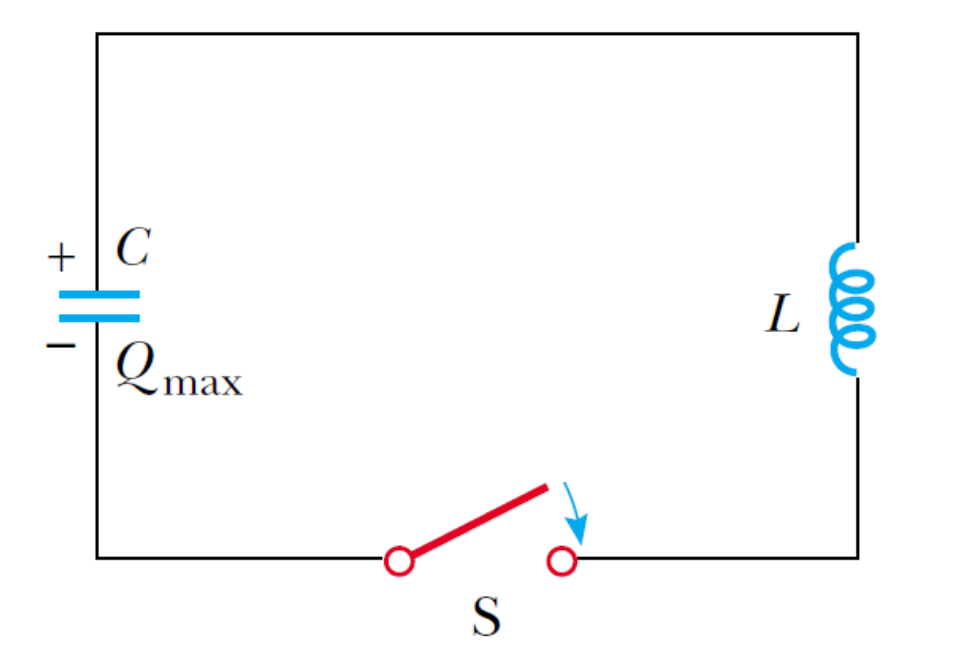
\includegraphics[scale = 0.275]{oz08/resources/Oz8Oef3.png}
\end{minipage}

% \begin{center}
%     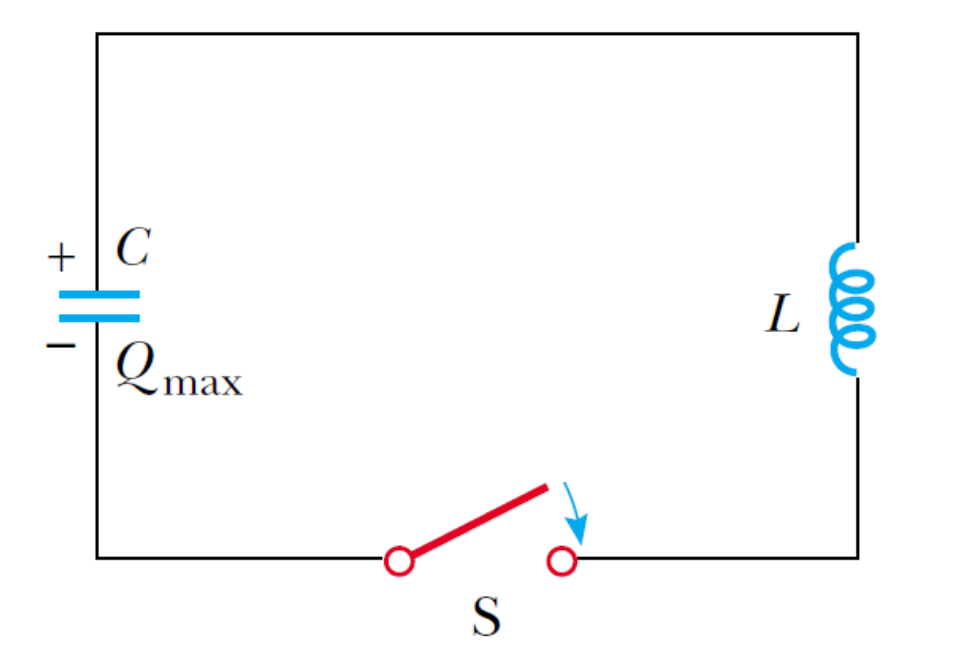
\includegraphics[scale = 0.3]{oz08/resources/Oz8Oef3.png}
% \end{center}


\begin{enumerate}[(a)]
    \item 
        \begin{description}[labelwidth=1.5cm, leftmargin=!]
            \item[Geg. :]   
            \item[Gevr. :] 
            \item[Opl. :]   
        \end{description}
    \item 
        \begin{description}[labelwidth=1.5cm, leftmargin=!]
            \item[Geg. :]   
            \item[Gevr. :] 
            \item[Opl. :]   
        \end{description}
    \item
        \begin{description}[labelwidth=1.5cm, leftmargin=!]
            \item[Geg. :]   
            \item[Gevr. :] 
            \item[Opl. :]   
        \end{description}
\end{enumerate}


\vspace{1cm}